% conteudo/teoria/integral_riemann.tex
% Definição formal da integral de Riemann

A integral de Riemann é um conceito matemático que formaliza o processo de
passagem ao limite das somas usadas para aproximar áreas.
Ela independe de interpretações geométricas sendo definida de forma puramente analítica.

\subsubsection{Partições e somas de Riemann}

A área do \textbf{círculo} (disco) pode ser aproximada particionando-se o disco em \(n\) triângulos,
cujos vértices estão no centro \(O\) e cujas bases são \textbf{cordas} consecutivas da
\textbf{circunferência}. Essa construção equivale a considerar um \textbf{polígono inscrito}
de \(n\) lados e decompor sua área em \(n\) triângulos.


À medida que tomamos mais triângulos (isto é, quando \(n\) aumenta), as cordas passam a aproximar
pequenos arcos da circunferência e a soma das áreas dos triângulos aproxima a área do círculo.

\medskip

Em cada triângulo, a \textbf{apótema} (segmento perpendicular do centro à base) coincide com a
\textbf{altura} do triângulo. Assim, a área do \(i\)-ésimo triângulo é
\[
A_i = \frac{b_i \, h_i}{2},
\]
em que \(b_i\) é o comprimento da corda (base) e \(h_i\) é a apótema correspondente.
Somando as áreas dos \(n\) triângulos, obtemos a aproximação
\[
A_n = \sum_{i=1}^{n} \frac{b_i \, h_i}{2}.
\]

\medskip

Quando \(n\) é grande, as apótemas \(h_i\) tornam-se cada vez mais próximas do raio \(r\).
Além disso, a soma das bases \(\sum_{i=1}^{n} b_i\) é o \textbf{perímetro} do polígono inscrito,
que tende ao comprimento da circunferência. Logo,
\[
A_n \approx \frac{1}{2} \left( \sum_{i=1}^{n} b_i \right) r
\quad\longrightarrow\quad
\frac{1}{2} \, (2\pi r) \, r = \pi r^2.
\]
Portanto, a área do círculo é
\[
A = \pi r^2.
\]

\medskip

\noindent\textbf{Nota (opção sem índices).}
Se tomarmos os \(n\) triângulos como \textbf{congruentes} (mesma base \(b\) e mesma apótema \(h\)),
então
\[
A_n = n \cdot \frac{b \, h}{2}.
\]
Nesse caso, \(n \cdot b\) é o perímetro do polígono inscrito e, quando \(n \to \infty\), temos
\(n b \to 2\pi r\) e \(h \to r\), concluindo novamente \(A = \pi r^2\).

% ===== DESENHO DO CÍRCULO =====
\begin{figure}[H]
  \centering
  \begin{tikzpicture}
    \def\R{3}
    \coordinate (O) at (0,0);

    % círculo (circunferência)
    \draw[thick] (O) circle (\R);

    % pontos nas extremidades dos raios
    \coordinate (A) at (60:\R);
    \coordinate (B) at (90:\R);
    \coordinate (C) at (120:\R);
    \coordinate (D) at (150:\R);

    % raios
    \draw[thick] (O)--(A);
    \draw[thick] (O)--(B);
    \draw[thick] (O)--(C);
    \draw[thick] (O)--(D);

    % cordas (lados do polígono inscrito)
    \draw[thick] (A)--(B)--(C)--(D);

    % marcar e rotular A,B,C,D
    \fill (A) circle (1.2pt) node[above right] {$A$};
    \fill (B) circle (1.2pt) node[above]       {$B$};
    \fill (C) circle (1.2pt) node[above left]  {$C$};
    \fill (D) circle (1.2pt) node[left]        {$D$};

    % --- apótemas (alturas) ---
    \coordinate (HAB) at ($(A)!(O)!(B)$);
    \coordinate (HBC) at ($(B)!(O)!(C)$);
    \coordinate (HCD) at ($(C)!(O)!(D)$);

    % hachura de um dos triângulos
    \fill[pattern=north east lines, pattern color=blue, opacity=0.3] (O)--(A)--(B)--cycle;

    % desenhar as apótemas
    \draw[thick, blue] (O)--(HAB);
    \draw[thick, blue] (O)--(HBC);
    \draw[thick, blue] (O)--(HCD);

    % marcar os pés e rotular
    \fill (HAB) circle (1.0pt) node[below right, xshift=-4pt, yshift=15pt] {$h_{AB}$};
    \fill (HBC) circle (1.0pt) node[below right, xshift=-15pt, yshift=20pt] {$h_{BC}$};
    \fill (HCD) circle (1.0pt) node[below right, xshift=-22pt, yshift=20pt] {$h_{CD}$};

  \end{tikzpicture}
  \caption{Triangulação por cordas e apótemas: a soma das áreas aproxima a área do círculo quando \(n\) cresce.}
\end{figure}

Se a mesma ideia for usada para uma \(f(x)\) no intervalo \([a,b]\), temos:


Dada uma partição $P$ do intervalo $[a,b]$ em $n$ subintervalos $[x_{i-1}, x_i]$, definimos a largura de cada intervalo como
\[
\Delta x_i = x_i - x_{i-1}.
\]
Para cada subintervalo, escolhe-se um ponto amostral $C_i \in [x_{i-1}, x_i]$. A soma
\[
\sum_{i=1}^{n} f(C_i) \, \Delta x_i
\]
é chamada de \textbf{soma de Riemann} associada à partição $P$.

Define-se ainda a \textbf{norma da partição} por
\[
\|P\| = \max_{1 \le i \le n} \Delta x_i.
\]
\begin{figure}[H]
  \centering
  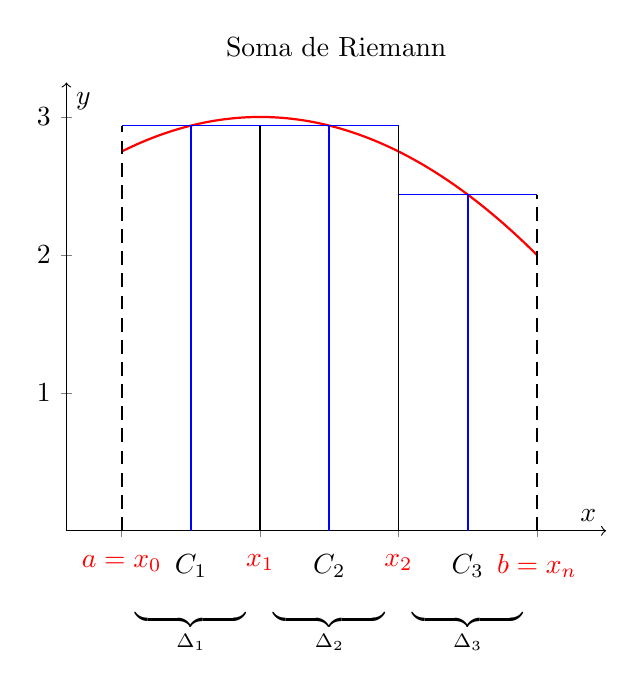
\begin{tikzpicture}
    \begin{axis}[
      xmin=0.3, xmax=2.25,
      ymin=0, ymax=3.25,
      axis x line=middle,
      axis y line=middle,
      axis line style={->},
      xlabel={$x$},
      ylabel={$y$},
      title={Soma de Riemann},
      clip=false,
      xticklabels={}
    ]
      % curva
      \addplot[red, thick, domain=0.5:2, samples=200] {2*x - x^2 + 2};

      % retângulos da soma
      \draw[dash pattern=on 5pt off 3pt, line width=0.6pt]  (axis cs:0.5,0) -- (axis cs:0.5,{2*0.75 - 0.75^2 + 2});
      \draw[blue, line width=0.6pt] (axis cs:0.75,0) -- (axis cs:0.75,{2*0.75 - 0.75^2 + 2});
      \draw[line width=0.6pt] (axis cs:1,0)    -- (axis cs:1,{2*0.75 - 0.75^2 + 2});
      \draw[blue, line width=0.6pt] (axis cs:1.25,0) -- (axis cs:1.25,{2*1.25 - 1.25^2 + 2});
      \draw[line width=0.6pt] (axis cs:1.5,0)  -- (axis cs:1.5,{2*1.25 - 1.25^2 + 2});
      \draw[blue, line width=0.6pt] (axis cs:1.75,0) -- (axis cs:1.75,{2*1.75 - 1.75^2 + 2});
      \draw[dash pattern=on 5pt off 3pt, line width=0.6pt]  (axis cs:2,0) -- (axis cs:2,{2*1.75- 1.75^2 + 2});
      % linhas de fechamento do topo
      \draw[blue, line width=0.6] (axis cs:0.5,2*0.75-0.75^2+2) -- (1,2*0.75-0.75^2+2);
      \draw[blue, line width=0.6] (axis cs:1,2*1.25-1.25^2+2) -- (1.5,2*1.25-1.25^2+2);
      \draw[blue, line width=0.6] (axis cs:1.5,2*1.75-1.75^2+2) -- (2,2*1.75-1.75^2+2);

      % marcas no eixo x
      \node[below, text=red] at (axis cs:0.5,-0.11) {$a=x_0$};
      \node[below, text=black] at (axis cs:0.75,-0.1) {$C_1$};
      \node[below, text=black] at (axis cs:0.75,-0.5) {$\underbrace{\hspace{4em}}_{\Delta_1}$};
      \node[below, text=red] at (axis cs:1,-0.1) {$x_1$};
      \node[below, text=black] at (axis cs:1.25,-0.1) {$C_2$};
      \node[below, text=black] at (axis cs:1.25,-0.5) {$\underbrace{\hspace{4em}}_{\Delta_2}$};
      \node[below, text=red] at (axis cs:1.5,-0.1) {$x_2$};
      \node[below, text=black] at (axis cs:1.75,-0.1) {$C_3$};
      \node[below, text=black] at (axis cs:1.75,-0.5) {$\underbrace{\hspace{4em}}_{\Delta_3}$};
      \node[below, text=red] at (axis cs:2,-0.1) {$b=x_n$};
          \end{axis}
  \end{tikzpicture}
  \caption{Aproximação da área sob $f(x)=2x-x^2+2$ por retângulos.}
\end{figure}
\subsubsection{Definição de integral de Riemann}

Dizemos que a função $f$ é \textbf{integrável no sentido de Riemann} em $[a,b]$
se existe o limite
\[
\lim_{\|P\| \to 0} \sum_{i=1}^{n} f(C_i) \, \Delta x_i,
\]
e esse limite é o mesmo para qualquer escolha dos pontos $C_i$ nos subintervalos.
Quando esse limite existe, ele é chamado de \textbf{integral definida de Riemann}
de $f$ em \([a,b]\) e é denotado por
\[
\int_a^b f(x) \, dx.
\]

\subsubsection{Condições suficientes de integrabilidade}

\begin{theorem}[Condições Suficientes de Integrabilidade]
Seja $f:[a,b] \to \mathbb{R}$ uma função definida em um intervalo fechado e limitado.
Então $f$ é integrável no sentido de Riemann em $[a,b]$ se satisfaz pelo menos uma
das condições a seguir:
\begin{itemize}
  \item $f$ é contínua em $[a,b]$;
  \item $f$ é monótona em $[a,b]$;
  \item $f$ é limitada em $[a,b]$ e possui somente um número finito de pontos de
  descontinuidade.
\end{itemize}
\end{theorem}
